\chapter{尾侧前额叶皮层:搜寻目标} \label{chap:chap5}

尾侧前额叶皮层有助于通过显性注意力(眼球运动)和隐性注意力对食物和食物迹象等物体进行视觉搜索,它的连接解释了它如何执行这些功能。尾侧前额叶皮层,包括额叶视区,与视觉皮层的背侧流和腹侧流以及脑干动眼神经核都有联系。
明显的注意依赖于它与脑干动眼核的连接,直接或间接地通过上丘和基底神经节。
隐蔽注意力依赖于增强的感觉反应,这种反应是通过与视觉皮层以及其他感觉区域的相互作用来调节的。
在早期灵长类动物中,随着眶额皮层的颗粒状部分,尾侧前额叶皮层也在进化(第\ref{chap:chap2}章)。
这两个新区域一起导致了在精细分支生态位的杂乱环境中发现、关注和评估物体的改进。



\section{介绍}

在前一章中,我们认为眶额皮层根据当前的生物需求对物体赋值。
本章提出,尾侧前额叶皮层搜索这些物体,它是通过隐蔽地注意周围目标和将眼睛朝向这些目标来实现的。


本章的大部分内容都是关于视觉和眼球运动的,它们在脊椎动物历史的早期就已经进化出来了。
眼睛和眼外肌肉的证据出现在最古老的脊椎动物和前脊椎动物化石中,有些可以追溯到500多万年前\cite{Shu et al. 2003}。
但是灵长类动物在视觉和眼球运动方面有一些重要的创新,比如发展出了中央凹和三色视觉(第\ref{chap:chap2}章)。
如果我们的结论——尾侧PF皮层首先出现在早期灵长类动物身上——正确,那么它比中央凹和全彩视觉都要早:这是关于其功能的重要线索。


为了理解尾侧前额叶皮层,我们首先需要看看它的连接是如何允许灵长类的前额叶皮层使用眼球运动和隐蔽注意力来搜索食物等物体的。



\section{区域}

在猕猴中,尾侧前额叶皮层指的是位于弓状沟膝侧的皮层。
图\ref{fig:fig_5_1}描绘了它的位置。


\begin{figure}
	\centering
	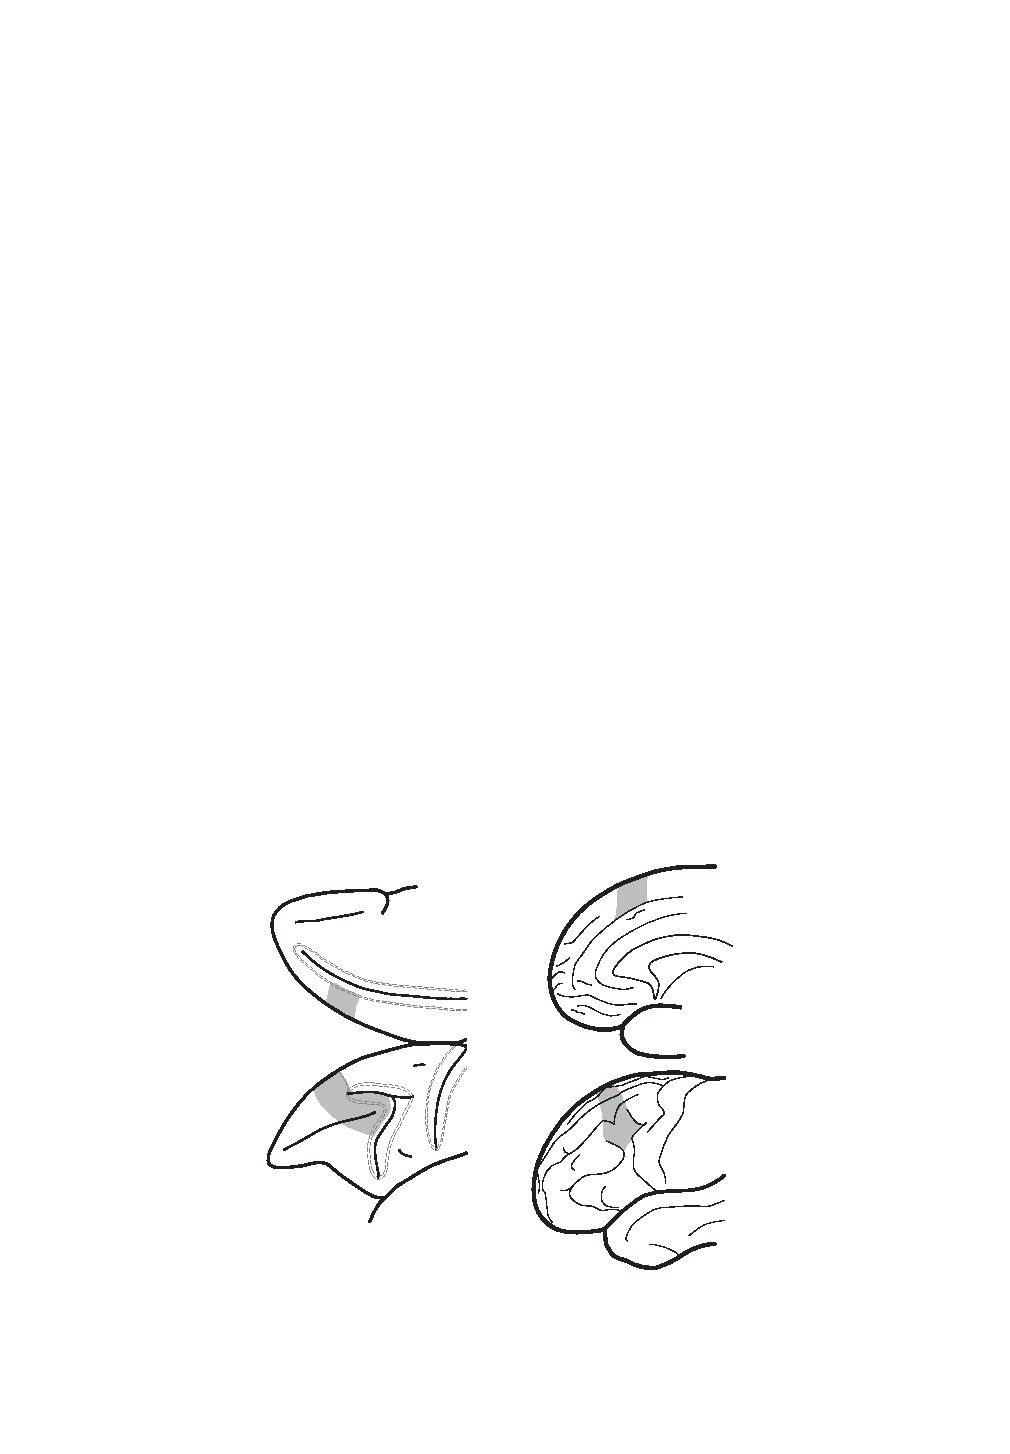
\includegraphics[width=0.7\linewidth]{image_pfc/Fig_5_1}
	\caption{猕猴(左)和人类(右)的尾侧PF皮层。格式如图\ref{fig:fig_1_2}所示。}
	\label{fig:fig_5_1}
\end{figure}


正如我们所定义的那样,尾侧前额叶皮层总是包括第8区,为了本章的目的,它还包括猕猴主沟的尾侧部分。
我们通过注意到,正如在第8区域\cite{Chafee & Goldman-Rakic 1998},主沟尾部的大多数细胞调节其活动与眼球运动相关\cite{Tanila et al. 1993}来证明这一分组是正确的。
Petrides和Pandya(1999)发现了一个位于主沟尾端附近的区域,他们称之为9/46,他们将该区域与相邻的吻侧中外侧PF皮层(46区)和背内侧9区区分开来。
顾名思义,Petrides和Pandya认为9/46区具有与9区和46区相似的细胞结构特性,并且这三个区域都具有颗粒状的细胞结构。
我们称主沟尾侧皮层为后外侧PF皮层(图\ref{fig:fig_1_4}),目前将其包括在PF尾侧皮层中。
然而,我们承认,在不违反任何解剖学原理的情况下,可以将其包括在前额叶皮层背侧(第\ref{chap:chap6}章)。
表\ref{tab:tab_1_2}使用一个查询标记(“?”)来表示这两个选项。
因此,关于后外侧前额叶皮层的许多观点都适用于本章和下一章。


在猕猴中,通过微刺激弓状沟靠近主沟尾端的吻侧岸,可以诱发眼跳运动\cite{Bruce et al. 1985},这一特性定义了额叶视区。
更高的电流可以通过电流传播,从更大的区域唤起跳视\cite{Robinson & Fuchs 1969},但人们普遍认为低阈值区域对应于额叶视区。
因此,区域8包括额叶视区,它从典型的颗粒状细胞结构向非颗粒状细胞结构变化\cite{Stanton et al. 1989}。


Amiez和Petrides(2009)回顾了通过电刺激在人脑中定位FEF的研究。
来自中央前上沟吻侧的低阈值刺激,以及来自中央前上沟上方的低阈值刺激,可以诱发眼跳。
Amiez等人(2006)使用成像方法来定位与个体受试者皮层解剖相关的激活峰值。
按照这样的定义,额叶视区始终位于中央前上沟的腹侧分支,这个位置与电刺激所定义的位置大致一致。
Amiez和Petrides(2009)提供了猕猴和人类的地图,并表明在这两种情况下,FEF都可以与运动前皮层区分开来,电刺激也可以唤起眼球运动。


微刺激还在猕猴的额叶中发现了第二个眼场:辅助眼场(SEF) \cite{Schlag & Schlag-Rey 1987}与FEF一样,SEF中的细胞在扫视前增加活动\cite{Hanes et al. 1995}。
在猕猴中,SEF位于背内侧额叶皮层的第6区\cite{Schlag & Schlag-Rey 1987;Olson & Gettner 1999},它在人脑中有类似的位置\cite{Amiez & Petrides 2009}。



\section{连接}

图\ref{fig:fig_5_2}显示了猕猴的尾侧前额叶皮层的皮质连接,包括额叶视区。
这些数据主要来自Petrides和Pandya(1999),他们将示踪剂注入区域8的细分(区域8B、8Ad或8Av),并描述了它们之间的联系。
这项研究比早期的研究更有优势(Petrides和Pandya 1984;Barbas 1988;Barbas和Pandya 1989;Cavada和Goldman-Rakic 1989), Petrides和Pandya(1999)进行了小规模和相对选择性的注射。


\begin{figure}
	\centering
	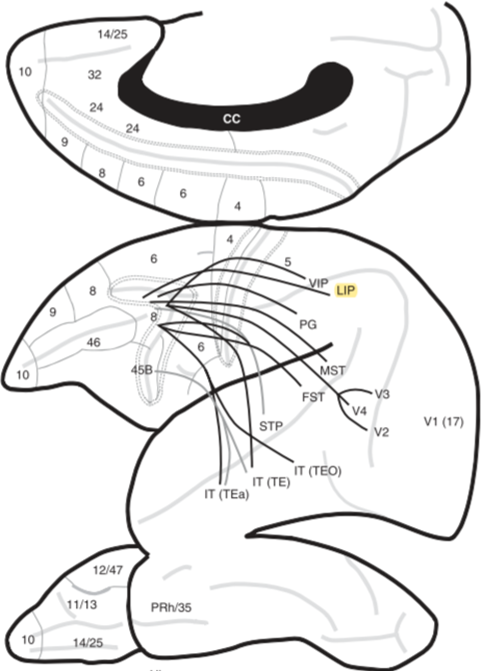
\includegraphics[width=0.7\linewidth]{image_pfc/Fig_5_2}
	\caption{末梢PF皮层的选定连接。图\ref{fig:fig_1_4}和\ref{fig:fig_1_5}给出了沟和区域的名称。这些线连接了一些与尾侧PF皮质有轴突直接连接的区域,除非另有说明,假设是相互的。}
	\label{fig:fig_5_2}
\end{figure}


根据连接得到以下结论:

\begin{enumerate}
	\item 8Ad区、8B区和后外侧前额叶皮层与执行眼肌运动和视觉空间功能的区域相连。例如,它们与位于顶骨内沟的LIP区有联系(Cavada和Goldman-Rakic 1989;Andersen等 1990), LIP中的细胞编码眼球运动(Snyder等 1997)。同样的PF区域与下顶叶皮层的PG区域有连接(Cavada和Goldman-Rakic 1989),该区域的许多细胞编码眼睛方向(Sakata等 1980)。最后,8Ad区与颞区MST区有联系,在MST区,细胞对视觉刺激的运动做出反应Celebrini和Newsome 1995)。
	\item 这些视觉区域构成了背侧视觉流的一部分(Ungerleider和Mishkin 1982;Milner和Goodale 2007),以区别于腹侧视觉流。一般来说,背侧流包括后顶叶区域,处理有关动作空间目标的信息,腹侧流包括颞下区域,处理有关视觉刺激的颜色、形状和纹理的信息。
	\item FEF接收早期(低阶)视觉区域的信息,如枕部视觉区V2和V3 (Stanton等 1995),但8Ad区和后外侧PF皮层不接收信息。因此,FEF接收到的高度处理视觉信息比PF皮层尾端的其他部分和PF皮层的其他部分要少。
	\item 8Av区不同于8Ad区、8B区和后外侧PF区,分别与腹侧流和背侧流有联系。8Av区与TEO区有联系(Webster等 1994),也与颞下皮层的其他部分有联系,如颞上沟下岸的皮层(Petrides和Pandya 1999)。
	\item 尾侧前额叶皮层各组成区域之间相互连接紧密。8Ad区和8Av区彼此相互投射,并与后外侧PF皮层(9/46区)相互投射。这些相互联系支持我们将后外侧皮层纳入本章。如图\ref{fig:fig_1_8}所示,我们所定义的尾侧前额叶皮层与Price和Drevets(2010)所定义的尾侧网络非常相似。
\end{enumerate}



图\ref{fig:fig_5_2}和前面的列表涉及皮质连接,但尾侧前额叶皮层的皮层连接也解释了其功能的一些重要内容:


\begin{enumerate}
	\item FEF (Künzle, 1976;Huerta等 1986)、8区其余部分(Fries 1984)和后外侧前额叶皮层(Selemon和Goldman-Rakic 1988)都向上丘发送直接投影。在所有脊椎动物中,上丘及其同源体都有定位头部感受器的功能。因此,这些皮质连接指向了尾侧PF皮层在控制眼球运动方面的作用,但大脑皮层的许多其他部分也投射到上丘(Leichnetz等 1981;Fries 1984),所以这种解剖特征并不能将PF皮层与其他区域区分开来。
	\item 额叶视区还可以通过向基底神经节的投射影响上丘的活动。额叶视区投射到尾状核的内侧(Stanton等 1988),后者又投射到黑质网状部(Hedreen和DeLong 1991)。该核投射到上丘,在那里发挥抑制作用(Hikosaka和Wurtz 1985)。
	\item 最后,额叶视区直接投射到脑干动眼肌核(Segraves 1992;Yan等 2001)。
\end{enumerate}



\subsection{总结}

尾侧前额叶皮层的连接指纹表明,它接受直接的、较低的视觉输入,它具有与背侧和腹侧视觉流平行的背侧-腹侧区别,并且它通过基底神经节到上丘的投射直接或间接地输出到动眼神经核。



\section{额叶视区是前额叶区域}

尽管有输出表明额叶视区在控制眼球运动中起作用,但我们并不认为额叶视区主要在眼球运动控制中起作用。
我们知道,当药物抑制额叶视区时,视觉引导的扫视在被引导到对侧空间时变得不准确(Sommer和Tehovnik 1997)。
在这个意义上,额叶视区类似于前运动皮层。
例如,腹侧前运动皮层的失活会导致肢体运动不准确(Kurata和Hoffman 1994)。


我们也知道额叶视区的永久性损伤不会消除眼跳运动,就像前运动皮层病变不会消除肢体运动一样。
然而,一个原因是除了其他区域外,SEF (Huerta和Kaas 1990)和顶叶区域LIP (Holloway 2002)也向上丘发送投射。
因此,为了消除眼跳,需要同时去除上丘和额叶视区(Schiller等 1979,1987)。只剩下最小的扫视。


然而,尽管有这些运动功能的证据,我们认为额叶视区是前额叶区域,而不是运动前区域。
我们这样做是因为我们区分了产生、发现和关注目标的机制和实现目标的机制。
记住,我们所说的目标指的是对象或地点,而不是奖励或结果。
实现目标的行动会产生结果。
除了在实验室,视觉注视和注意力永远不会产生这种意义上的结果。
在野外,看着或吃着一种食物并不会产生任何营养或补水的好处。
实现这一预期结果需要其他机制。我们认为前者是前额叶皮层的功能,后者是前运动皮层的范围。


Shadmehr和Wise(2005)在他们对前运动皮层的治疗中提出,它处理的是视运动转换,将伸手运动的视觉目标转换为关节角度和力的变化,从而驱动手到达这些目标。
第\ref{chap:chap2}章提到了这种机制。
详细信息可以在Shadmehr和Wise中找到,但这里有一个简短的总结。


假设有人伸手拿咖啡杯。
基本上,电机系统需要建立两个位置:目标位置和手的初始位置。
Shadmehr和Wise提出后顶叶和前运动皮层的细胞在一个坐标框架中编码这些位置,在其原点,视觉注视点。然而,在理论上,任何视网膜坐标都可以作为原点。
图\ref{fig:fig_5_3}显示了这种机制是如何工作的。
图中显示了两个向量:一个是尾巴在注视点,尖端在运动目标处;
另一种是尾巴在固定点,尖端在手的当前位置。
两个向量的简单相减就得到了一个向量,它的尾部在手上,顶端在目标上。这个计算的结果相当于一个“运动计划”,将视觉参考系转换为以手为中心的坐标系。
前运动区和初级运动区,连同皮层下结构,将这个矢量转换成关节角度的变化和使这个运动的力量。


\begin{figure}
	\centering
	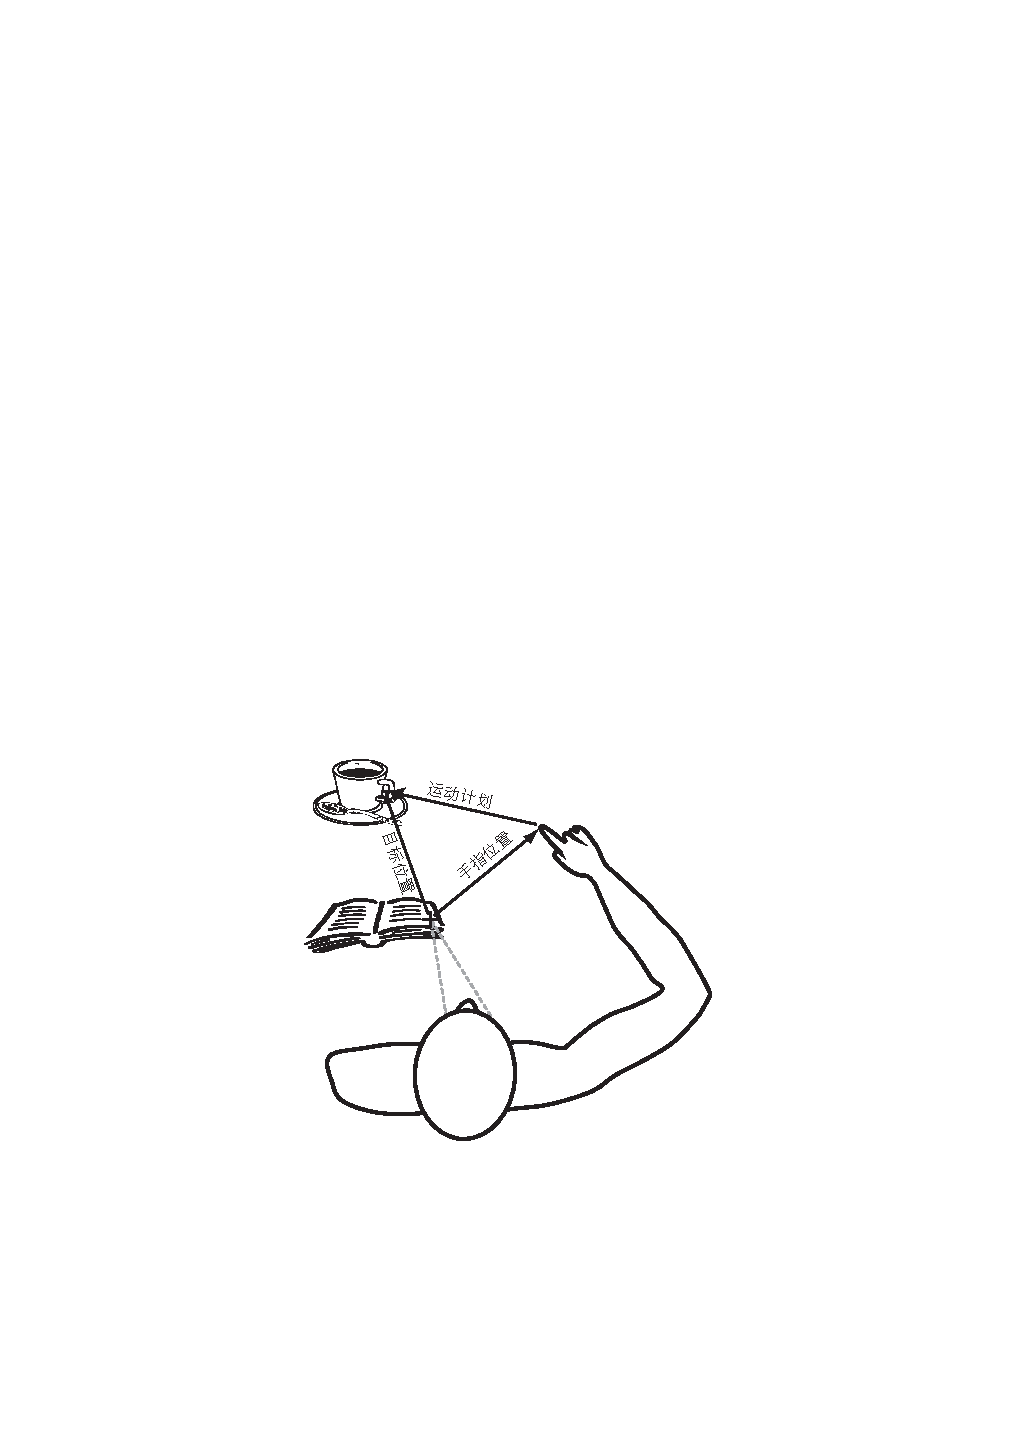
\includegraphics[width=0.7\linewidth]{image_pfc/Fig_5_3}
	\caption{运动平面的矢量表示。这个人的目标是把他的指尖穿过咖啡杯的把手。他或她制定了一个读书计划。“+”标志着他当时的注视点。来自注视点的两个向量编码目标的位置和手指在非中心的外部坐标框架中的当前位置:注视中心坐标。两个矢量之间的差表示以手为中心坐标的电机平面。修改自Shadmehr R, Wise SP.《触摸和指向的计算神经生物学:运动学习的基础》,©2005麻省理 工学院,经麻省理工学院出版社许可。}
	\label{fig:fig}
\end{figure}


通过这种机制或类似的机制,前运动区和后顶叶区以一种眼球运动或其他形式的注意力都无法实现的方式实现目标。
在我们的例子中,这个人想要咖啡,所以把他或她的注意力转移到杯子上。
注意力可以是显性的,即中央凹朝向杯子,也可以是隐性的,即只关注杯子而不看它。
杯子里的东西与人当前的需求有关,因此他或她产生了一个目标——咖啡杯——然后搜索并将注意力转移到杯子上。
我们认为,尾侧前额叶皮层执行搜索和注意功能。
虽然视觉固定和注意力不能达到预期的结果,但伸手到杯子里,把它送到嘴里,从里面喝水就可以了。
我们将后一种功能视为前运动区和初级运动区,以及运动系统的其他部分。


那么,有什么证据表明额叶视区参与了对目标的寻找和关注,而不是实现目标的手段?
我们已经看到,与运动前区域不同,额叶视区接收来自低阶视觉区域的直接输入,特别是枕叶和颞叶皮层称为V2、V3、V4和MST的区域(Stanton等 1995)。
这些联系解释了为什么额叶视区中的一些细胞在感觉刺激出现后表现出活动增加,而在运动之前却没有(Schall 1991)。
它们似乎明确了视觉目标,而不是注视这些目标所需的眼球运动。
此外,在顶叶区LIP投射到FEF的细胞中,78\%有视觉反应,但没有扫视相关活动(Ferraina等 2002)。
这种投影可以提供另一种关于视觉目标的信息来源,而且是独立于运动指令的信息来源。


当然,额叶视区中的许多细胞具有视觉运动活动:它们在视觉目标出现时和眼球运动之前调节自己的活动(Schall 1991)。
其中很多都是在刺激出现后不久,即刺激引起注意时,指定刺激的位置。
Sato和Schall(2003)教猴子在一系列干扰物中发现一个视觉弹出刺激,然后对该位置进行扫视(prosaccade试验)或对相反方向的扫视目标进行扫视(反扫视试验)。
如果活动反映了刺激的位置,那么两种试验类型的活动应该是相同的。


Sato和Schall比较了两项任务中FEF细胞的活动,当弹出的刺激落入细胞的接受野时。
对于反眼跳任务,注意当弹出刺激这样做时,眼跳目标是在相反的方向。
然而,57\%的任务相关细胞的活动最初反映了刺激的位置,尽管随后86\%的这些细胞后来编码为扫视目标。


这些结果表明,额叶视区中的细胞活动可以反映刺激的位置,独立于运动,并且这种活动反映了隐蔽注意的方向。
与这一观点一致,Armstrong和Moore(2007)表明,额叶视区的皮质内微刺激增强了视觉区V4(腹侧视觉流的中层区域)的细胞反应。
它是专门为视觉空间的一个特定部分做的。
刺激FEF的效果可能模仿了猴子在该位置秘密关注物体时所发生的情况。


如果FEF真的在隐性注意和显性注意中起作用,该区域的暂时失活应该会导致对中央凹外刺激的注意受损。
因此,Wardak等(2004)教猴子在干扰物中发现目标,而动物则保持对中心光点的固定。
在额叶视区失活后,猴子发现周围目标的速度很慢。
Iba和Sawaguchi(2003)表明,失活也会导致猴子对目标进行扫视的速度变慢。
这些发现表明,额叶视区在对刺激的公开注意和隐蔽注意中都有作用,特别是当这些刺激作为后续行动的目标时。


这一观点与第\ref{chap:chap2}章中关于前额叶进化的描述非常吻合。
Strepsirrhine灵长类动物没有中央凹,早期灵长类动物可能也没有。
因为包括额叶视区在内的尾侧前额叶皮层在早期灵长类动物中进化而来,它一开始不可能与中央凹或中央凹有任何关系。
所以,从这个意义上说,这些动物的所有视觉都对应于中央凹外视觉,所有的注意力都是隐蔽的。
顺畅的眼球运动可以让类人猿灵长类动物锁定中央凹,将注意力集中在移动的物体上,并保持高分辨率图像。
但这种能力也可能在缺乏中央凹的灵长类动物中进化而来(Shepherd和Platt 2010)。
因此,从中央凹视觉或明显的注意力来解释灵长类动物的前额叶皮质的起源是错误的,尤其是尾前额叶皮质的起源。


然而,中央凹最终在后来的灵长类动物中进化出来,现代眼镜猴、猴子、猿和人类(单足纲)通过遗传拥有它。
尽管有很多优点,但集中注意力的能力是有代价的。
那视觉世界的其余部分呢?
这个混乱的世界还包含许多其他突出的项目。
在某种意义上,没有中央凹的视网膜提供了一个更平衡的世界观。
即使在中央凹进化之后,保持隐蔽注意力的好处是,它可以增强对有限数量的中央凹外物体的处理,即使最密集的处理是用于中心凹的物体和地方。
隐蔽注意力和搜索的重要性在于,所有被关注的对象,而不仅仅是被聚焦的对象,都可能成为未来行动的目标。
根据这一观点,包括FEF在内的尾侧PF皮层进化为隐蔽的搜索和注意力,但后来一旦中央凹出现,就适应了公开的注意力。



\subsection{总结}

许多神经科学家将额叶视区视为眼球运动区域,并将其视为眼球运动的前运动区域。
我们提出一个不同的想法。
我们将额叶视区和尾侧前额叶皮层的其他部分视为前额叶区域,而不是前运动区域,并提出它们在寻找和关注灵长类动物重要目标方面发挥作用。
在许多灵长类动物中,包括猴子和人类,对目标的关注通常意味着眼球运动,使中央凹朝向目标(扫视)或在目标移动时保持视觉固定(平稳追求)。
但是隐蔽的注意力也扮演着重要的角色,在缺乏中央凹的早期灵长类动物中,它肯定是这样的。
由于注视是注意力的一种形式,我们将眼球运动视为一种注意力功能,而不是一种运动功能。
我们提出,包括额叶视区在内的尾侧前额叶皮层的功能是将公开或隐蔽的注意力引向一个目标,而不是作为实现目标的机制的一部分。



\section{动眼肌延迟反应任务}
我们将FEF与PF尾部皮层的其余部分分开处理,因为FEF的皮质内微刺激会引起眼球运动。但是,正如在连接部分所解释的那样,FEF与尾侧PF皮层的其他部分有紧密的连接。因此,8区(Chafee和Goldman-Rakic 1998)和后外侧PF皮层(Funahashi等 1989)的许多细胞具有与眼球运动相关的活动。

正如我们前面所说的,后外侧PF皮层的连接使我们在本章中将其与包括FEF在内的后外侧PF区一起考虑。我们在第\ref{chap:chap2}章中对皮层进化的讨论为这种方法提供了一些可信度,后外侧PF皮层中存在编码眼球运动的细胞。由于后外侧前额叶皮层(9/46区)处于中间状态,在本节中,我们将讨论在第\ref{chap:chap6}章中再次出现的主题,最显著的是被称为“空间记忆任务”的任务中的延迟期活动问题。我们这样做主要是为了方便,并认为没有什么关键取决于我们是否将后外侧PF皮层与PF区的尾侧组或背侧组进行分类。

动眼力延迟反应任务在包括后外侧PF皮层在内的尾侧PF皮层的研究中发挥了突出作用。它不同于经典的延迟反应任务,因为猴子通过扫视而不是到达一个空间目标来选择潜在的目标。

\begin{figure}
	\centering
	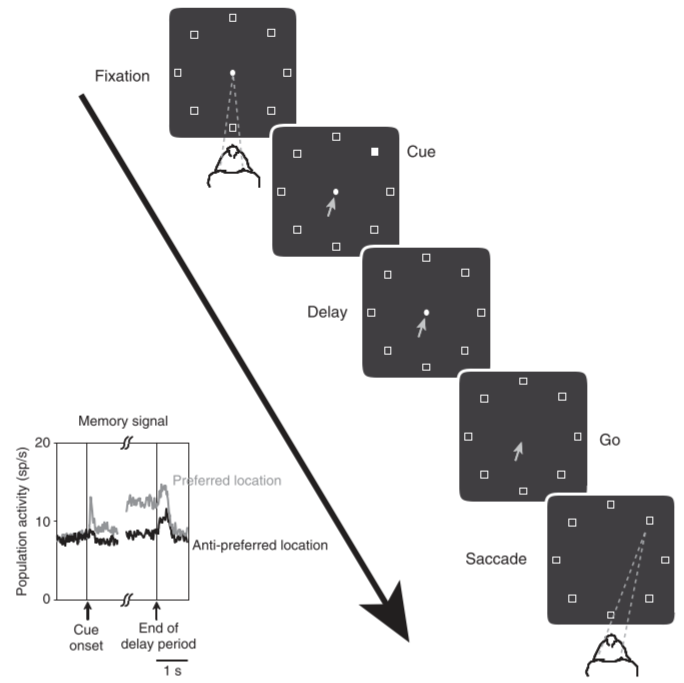
\includegraphics[width=0.7\linewidth]{image_pfc/Fig_5_4}
	\caption{普通版本的动眼器延迟反应任务。在试验过程中,每个面板在不同的时间显示屏幕,在其他试验中,未填充的白色方块是潜在的空间目标。填满的白色方块表示一个例子试验的线索,填满的白色圆圈表示注视点。灰色虚线和灰色箭头表示猴子的注视点。左下方的插入图显示了空间记忆信号,由Lebedev等人(2004)从PF皮层细胞群中记录,灰色为首选记忆位置的平均活动,黑色为反首选位置的平均活动。因为Lebedev等人控制了注意力,这些数据代表了PF皮层空间记忆信号的最有力证据,尽管它们只出现在延迟期间编码位置的少数细胞中。}
	\label{fig:fig_5_4}
\end{figure}

动眼肌延迟反应任务有三个阶段:提示、延迟和选择(图\ref{fig:fig_5_4})。在第一阶段,一个视觉空间线索会短暂地出现在受试者视野的某个地方。这个刺激指示了猴子必须扫视的位置,但直到延迟期结束,猴子必须继续盯着一个中心光点。在一段从几百毫秒到几秒不等的延迟时间后,一个“开始”信号告诉受试者将扫视移动到最近提示的位置。如果被试的扫视准确,就会得到奖励。

尽管实验人员可以使用任何提示位置的配置,但常见的版本包括以注视点为中心等距排列的八个显著位置,如图\ref{fig:fig_5_4}所示。该图将位置显示为空方格,并表示球杆为填充方格。然而,重要的是要注意,正如通常所呈现的那样,外围位置没有以任何方式标记,这意味着当猴子响应“go”信号时,它会扫视到屏幕上未标记的位置。

在这项任务中,尾侧和后外侧前额叶的许多细胞表现出延迟期活动(Chafee和Goldman-Rakic 1998)。图\ref{fig:fig_5_4}显示了Lebedev等人(2004)在种群水平上从尾侧PF皮层记录的记忆信号。

Funahashi和他的同事(Funahashi等 1989;Takeda和Funahashi 2002)展示了他们的电极穿透皮层的位置图,我们假设这些细胞延伸到整个采样区域。Lebedev等人的研究表明,具有记忆特异性信号的细胞位于主沟尾端9毫米处,主要位于主沟背侧及其附近。Chafee和Goldman-Rakic(1998)报告说,延迟期活动主要来自8A区,但他们的图表显示,一些细胞也来自后外侧PF皮层。

成像实验在类似领域也得到了结果。Inoue等(2004)比较了眼肌运动延迟反应任务中的眼跳激活与猴子对屏幕上标记的位置进行眼跳的任务中的激活。差异激活位于后外侧PF皮层和8区,包括FEF。

鉴于以下事实,这是一个重要的观察,下一章将解释,在经典的、达到版本的延迟反应任务上的表现取决于中外侧PF皮层,而不是尾侧PF皮层。因此,动眼肌延迟反应任务不同于经典的延迟反应任务,基于动眼肌版本任务的结论不一定适用于经典的延迟反应或延迟交替任务。后外侧前额叶损伤对这些任务的经典版本缺乏影响(Butters和Pandya 1969),这强化了这样一种观点,即该区域在目标的寻找和关注中发挥作用,而不是在目标的实现(前运动皮层功能)或目标的产生(背侧前额叶皮层功能,如第\ref{chap:chap6}章所述)。

\begin{figure}
	\centering
	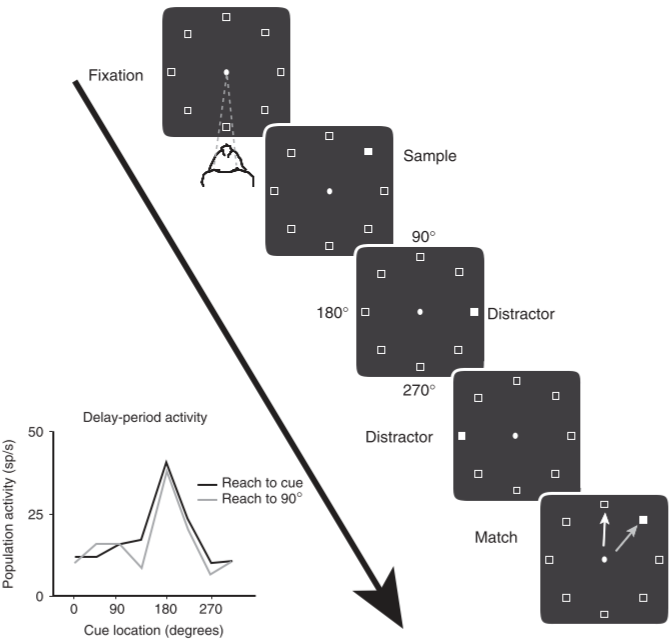
\includegraphics[width=0.7\linewidth]{image_pfc/Fig_5_5}
	\caption{di Pellegrino和Wise(1993)使用的空间匹配样本任务。格式如图\ref{fig:fig_5_4}所示。在底部面板上,箭头表示在两种情况下达到运动的目标。在一种情况下,提示的位置是伸手动作的目标;在另一种情况下,无论球杆的位置如何,90°的位置(图中向上)始终是到达目标。左下方的插图显示了PF皮层中一个细胞的活动,该细胞在延迟期间编码最左边的线索(180°),在两种情况下都是一样的。}
	\label{fig:fig_5_5}
\end{figure}

\subsection{解释延迟期活动}
传统的解释是,眼肌运动延迟反应任务中的延迟期活动,就像延迟反应任务的标准版本一样,反映了回溯性空间工作记忆。根据这种观点,这种活动反映了在短期记忆中线索位置的维持。这种解释部分来自于将该任务称为“空间记忆任务”,并因此假设在延迟期间发生的主要认知过程是感官信息的维持。事实上,这种观点的支持者经常把延迟期称为“记忆期”。但是,第\ref{chap:chap1}章警告不要接受任务的名称。事实上,在延迟期间还会发生其他过程,包括对提示位置的隐蔽注意和运动的准备。

有几种方法可以区分这些可能性,我们将它们进行了编号:

\begin{enumerate}
	\item 我们可以比较动眼肌延迟反应任务的两个版本。因此,Funahashi等人(1993b)比较了一个版本,其中猴子必须对目标进行扫视(prosaccade),另一个版本中猴子必须对距离线索180°的位置进行扫视(反扫视)。在后来的一项研究中,Takeda和Funahashi(2002)比较了标准的动眼肌延迟反应任务和猴子必须以90°的角度扫视该位置的条件。
	
	这些实验有如下逻辑:如果延迟期活动编码了线索在记忆中的位置,那么无论运动的目标是什么,它都应该是相同的。在这两项研究中,大多数与任务相关的细胞反映了线索的位置,尽管有相当一部分反映了目标的位置。Funahashi等人报告说,51个与任务相关的细胞中有31个(61\%)编码了线索的位置,而这51个细胞中有13个编码了目标的位置。尽管细胞样本很小,但这些发现使作者得出结论,延迟期活动反映了对提示位置的记忆。
	\item 第二种方法试图排除这种可能性,即通过使用单一的、重复的手部运动来报告线索的位置,而不是移动到该位置,从而对非感官因素进行编码。Sawaguchi和Yamane(1999)使用了这种方法。他们在延迟期后呈现一个空间视觉线索,并要求猴子只有在与线索位置匹配的情况下才释放杠杆。读者会认为这是匹配样本任务的空间版本。在与任务相关的神经元中,48\%显示出延迟期活动,这些细胞中90\%编码了提示位置。这些结果也被用来支持延迟期活动在空间记忆方面的解释。
	\item 正如di Pellegrino和Wise(1993)所做的实验那样,上述两种方法可以结合起来。实验设计如图\ref{fig:fig_5_5}所示。在Sawaguchi和Yamane(1999)的实验中,猴子需要报告延迟期结束时的线索是否与延迟前出现的线索的位置相匹配。然而,猴子以不同的方式报告匹配的刺激,如图\ref{fig:fig_5_5}底部的两个箭头所示。这种报告要求从一个试验块到下一个试验块交替进行。在一个街区,猴子向提示的位置移动。在下一个街区,不管线索和匹配的刺激出现在哪里,猴子都到达一个固定的位置。有时,提示方向和报告方向之间的夹角等于180°,如Funahashi等人(1993b)的反眼跳任务,有时等于90°,如Takeda和Funahashi(2002)的实验。
	
	Di Pellegrino和Wise记录了尾侧和后外侧PF皮层,并发现,与Funahashi等人一样,无论运动的目标如何,61\%的细胞具有相同的延迟期活动(图\ref{fig:fig_5_5})。这一结果也可以表明,细胞的活动编码了对提示位置的记忆。
	\item 所有这些研究都基于这样一个假设:只有两个重要因素是线索的位置和移动目标的位置。将延迟期称为“记忆期”,人们很容易忽略另一种可能性,即与记忆一样,延迟期也涉及注意力:有时是显性的,有时是隐性的。为了测试这种可能性,Lebedev等人(2004)引入了一种新的实验设计,如图\ref{fig:fig_5_6} A所示。正如第\ref{chap:chap1}章所提到的,他们教猴子记住一个空间位置,并秘密地注意到另一个位置,同时这样做。
	
	Lebedev等人记录了尾侧和后外侧PF皮层的细胞活动。在对空间位置进行编码的任务相关细胞中,大多数(61\%)选择性地对参与的位置进行编码,而不是对记忆中的位置进行编码。少数(16\%)细胞选择性地编码记忆位置,其他细胞具有中间属性(图\ref{fig:fig_5_6} B)。注意信号在每个测量中都超过了记忆信号(图\ref{fig:fig_5_6} C)。
	\item 如果大多数细胞反映隐蔽注意力,那么当受试者需要参加某个地方,但不需要记住这个位置时,就应该有可能证明激活。成像可以用来检验这一预测。Astafiev等(2003)提示受试者在保持中心注视的同时注意左边或右边。他们报告了FEF的激活,以及在顶骨内沟附近的后顶骨区域。
	
	Curtis和D’esposito(2006)进行了类似的成像研究,但有两次延迟。他们的实验对象看到了即将到来的扫视的几个潜在目标,随后是第一个延迟期,在此期间,实验对象需要记住这些地方。在第一次延迟期间,FEF和后顶叶皮层都发生了持续的激活。然后出现了一个箭头,指示在该试验中哪个目标应该是眼球运动的目标。第二次延迟后,受试者按指示进行扫视。在第二次延迟期间,持续的激活只发生在FEF,而不是在后顶叶皮层。这一发现与中央凹是一种注意力功能的观点一致。包括FEF在内的尾侧PF皮层,在将注意力导向潜在目标方面发挥作用,这在两次延迟期间都发生过混乱,不仅仅是在记忆位置上,发生在第一次延迟的时候。
\end{enumerate}
\begin{figure}
	\centering
	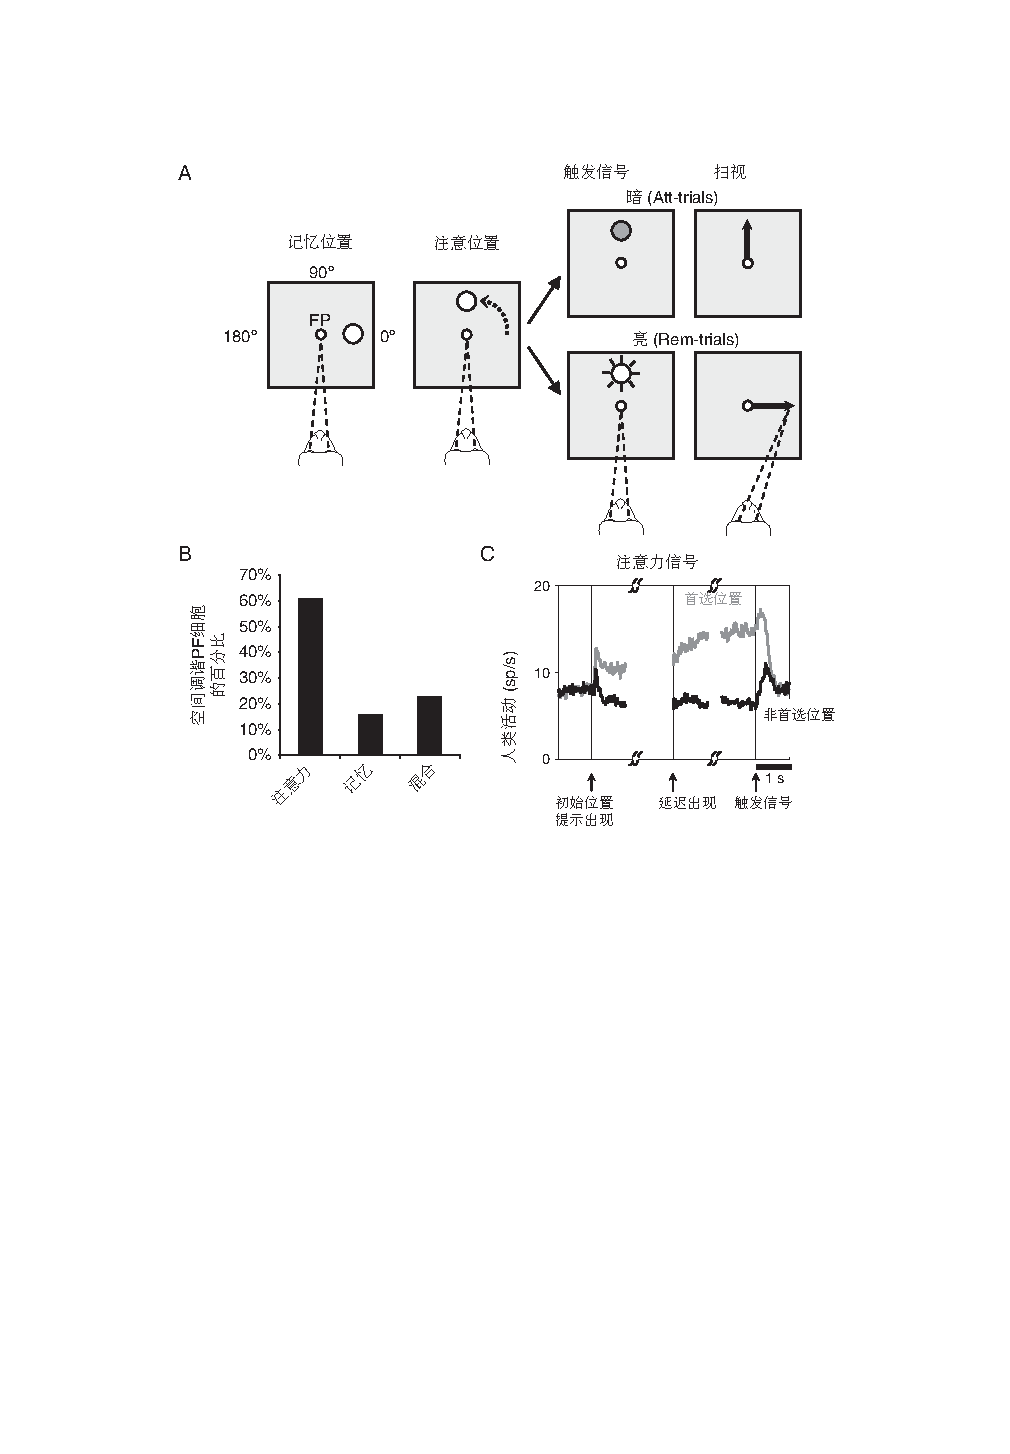
\includegraphics[width=0.7\linewidth]{image_pfc/Fig_5_6}
	\caption{PF皮层的注意力和记忆编码。(A)任务设计。视频监视器上出现一个圆(灰色矩形),随后开始围绕中心注视点(FP)旋转。它从四个位置中的一个开始,然后停在相同的四个位置中的一个:从中心向上、向下、向左和向右。如果圆圈变暗(上叉),猴子需要在这次试验中扫视圆圈的最终位置;如果它变亮了(底部的叉子),猴子必须在这次试验中向圆圈的初始位置扫视。箭头表示在两种情况下正确的扫视。缩写:Rem,记忆位置;丙氨酸,attended-location。(B)空间调谐的PF皮层神经元编码参与或记忆的位置或两者(混合)的百分比。(C)注意信号格式为记忆信号,如图\ref{fig:fig_5_4}所示。(A)转载自Lebedev MA, Messinger A, Kralik JD, Wise SP.前额叶皮层中参与位置与记忆位置的表示。PLoS Biology 2:1919-35,©2004公共科学图书馆,经许可。}
	\label{fig:fig_5_6}
\end{figure}

我们得出结论,在这些实验中,延迟期活动或激活有几种可能的解释。它可以反映对提示位置的记忆,对该位置的隐蔽注意力,或将公开注意力引导到该位置的准备。此外,它还可以反映任务规则的编码,这是我们将在下一章讨论的主题。

因此,动眼肌延迟反应任务延迟期间的活动并没有显示任何关于回顾性空间工作记忆的内容。首先,这种活动反映的是隐蔽注意力,而不是感官记忆。第二,工作记忆的概念没有区分位置的回顾编码和前瞻性编码。正如我们在下一章所解释的那样,前瞻性编码一词指的是对选定目标的短期记忆。尽管一些实验,如Funahashi等人的反眼跳任务,试图排除目标位置的预期编码,但在每种情况下,都有相当数量的少数细胞编码目标。将空间注意力与空间记忆进行对比的实验表明,PF皮层的大部分活动编码的是隐蔽参与的位置,而不是被记住的位置。我们将在第\ref{chap:chap6}章和第\ref{chap:chap7}章回到前瞻性编码的主题。
\subsection{中断延迟期活动}
不管对延迟期活动的正确解释如何,中断它都会造成某种程度的损害。然而,简单地表明,在尾叶前额叶皮层有损伤的猴子在一项任务中表现得很差,并不能证明它们这样做是因为它们不再记得提示的位置。这也可能表明他们很难注意到提示的位置或在记忆中保持它的预期代码。

受试者在动眼肌延迟反应任务中可能会犯两种类型的错误。Frank误差涉及错误的空间目标的选择(Keller等 2008),而精度误差涉及更接近正确目标而不是任何其他可能目标的移动,但错过了其确切位置。

不准确的扫视可能反映了低水平的运动障碍,因此需要将缺乏延迟期的控制条件与标准任务进行比较。在这里,受试者只是对一个可见的目标进行扫视。

猴子的FEF失活会引起低视眼跳。也就是说,对可见位置的扫视往往达不到空间目标(Dias和Segraves 1999)。低眼跳也发生在FEF单侧病变的患者中(Gaymard等 1999;Ploner等 1999)。

冷却导致8A区失活也会导致眼球运动延迟反应任务的不准确扫视。他们往往达不到正确的目标位置,或在目标位置的一侧(Chafee和Goldman-Rakic 2000)。用肌西酚(Sawaguchi和Iba 2001)或多巴胺拮抗剂(Sawaguchi和Goldman-Rakic 1991)灭活后外侧PF皮层具有同样的效果。后外侧PF皮层的单侧消融也是如此(Funahashi等 1993)(图\ref{fig:fig_5_7})。

尽管FEF、尾侧PF皮层的其他部分或后外侧PF皮层的失活会导致不准确的扫视,但这些扫视通常朝着正确的方向前进,并在更接近提示位置的地方结束,而不是任何其他目标。然而,Funahashi等人(1993a)得出结论,这些眼跳的不准确反映了回溯性空间工作记忆的失败。

他们从未解释过,如果猴子不记得目标位置,它们的扫视最终会更接近提示的位置,而不是任何其他潜在的目标位置。
\begin{figure}
	\centering
	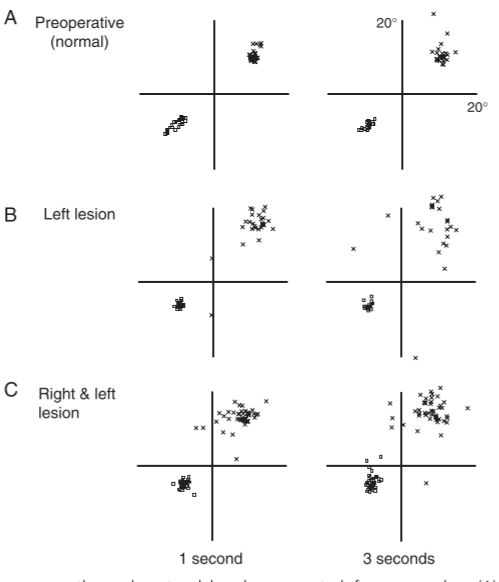
\includegraphics[width=0.7\linewidth]{image_pfc/Fig_5_7}
	\caption{一只猴子在动眼力延迟反应任务上的表现。(A)术前(正常)表现正方形表示225°(向下和向左)目标的扫视终点;十字表示45°(向上和向右)的目标。(B)左半球后外侧PF皮层单侧损伤后的表现。(C)右半球同一区域额外病变后的表现,以完成双侧病变。底部的延迟持续时间。摘自Funahashi S, Bruce CJ, Goldman-Rakic PS背外侧前额叶病变和动眼肌延迟反应表现:记忆性“盲点”的证据。神经科学杂志13:1479-97,©神经科学学会,1993年,经许可。}
	\label{fig:fig_5_7}
\end{figure}

工作记忆解释的支持者可能会争辩说,猴子之所以不会犯明显的错误,是因为这些损伤,无论是永久性的还是暂时性的,都是单方面的。毕竟,我们知道在标准延迟反应任务中,中外侧前额叶皮层的单侧损伤只会引起轻度损伤(Rosen等 1975),而双侧损伤后的损伤是严重的(Goldman等 1971)。因此,Funahashi等人(1993a)在两只猴子身上进行了双侧损伤,并分两个阶段进行。图\ref{fig:fig_5_7}显示了其中一种动物的数据。这只猴子在第二次损伤后有更大的损伤,但大多数扫视仍然在目标位置附近结束(图\ref{fig:fig_5_7})。病变很少引起明显的错误。在6秒的较长延迟(未显示)下,眼跳端点比较短延迟时分布得更广,但猴子犯准确错误的频率仍然比坦率错误高得多。

话虽如此,我们并不否认,PF皮层受损或失活的猴子有时确实会犯明显的错误。但是,对猴子在犯下明显错误后的行为的研究表明,这种损伤与回溯性工作记忆几乎没有关系。Tsujimoto和Postle(2012)报道了PF中外侧皮层(46区)失活的影响,所以我们在下一章中再次讨论。这些失活在动眼肌延迟反应任务上造成了明显的错误。在猴子犯了这样的错误后,它们的第一次扫视和下一次扫视都瞄准了适当的目标(图\ref{fig:fig_5_8})。这一发现表明,猴子并没有忘记线索的位置或适当目标的位置。
\begin{figure}
	\centering
	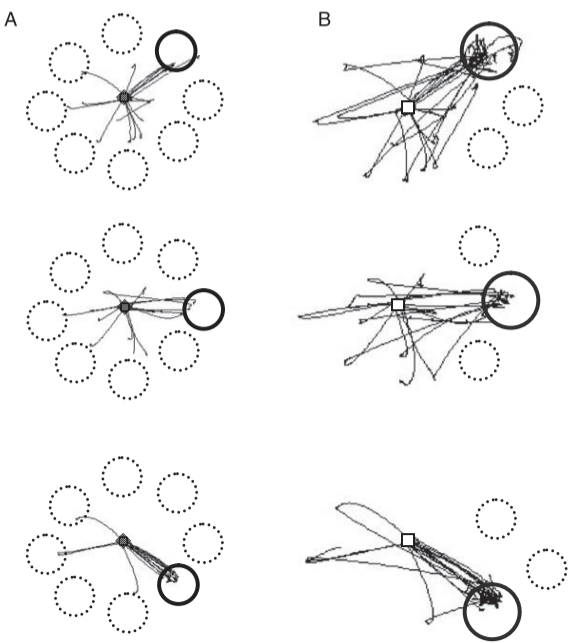
\includegraphics[width=0.7\linewidth]{image_pfc/Fig_5_8}
	\caption{在一个明显的错误后的纠正性扫视。(A)在中外侧PF皮层失活后,猴子对错误的目标进行了一些扫视。对于图的顶部部分,正确的目标是右上方的位置,对于中间部分,正确的位置,对于底部部分,正确的位置是右下方的位置。(B)对一次不正确扫视的直接后果的检查表明,猴子在那次试验中对适当的目标进行了矫正扫视。修改自Tsujimoto S, Postle BR。前额叶皮层和动眼肌延迟反应:记忆性盲点的重新思考。认知神经科学杂志24:627-35,©2012由麻省理工学院}
	\label{fig:fig_5_8}
\end{figure}
辻本和波斯特尔还分析了坦率错误的模式,发现猴子经常选择在前一次试验中合适的目标并获得奖励。因此,很明显,猴子在回溯性空间工作记忆方面并没有简单的损伤。相反,正如我们在下一章中提出的那样,有PF皮层损伤的猴子在区分之前的目标和当前的目标方面有缺陷。

因此,干扰延迟期活动的证据并不支持损伤导致回溯性感觉记忆丧失的观点。相反,它表明病变干扰了对未标记位置的扫视的准确性,以及区分以前目标和当前目标的能力。尾侧前额叶受损的猴子似乎保留了正确目标的知识,但很难将这种知识转化为准确的扫视。
\subsection{消除延迟期}
延迟期线索的缺乏导致了延迟期活动反映线索记忆的假设:回顾性空间记忆。如果是这样,并且如果回溯性空间记忆是尾侧PF皮层的关键功能,那么我们可能会认为在没有延迟期的任务中活动减弱。更重要的是,尾侧PF皮层的损伤不应该导致对缺乏记忆要求的任务的损害。实验结果与这两种观点都不相符。

戈尔德和沙德伦(2007)向猴子展示了一个由移动的圆点组成的线索。这些点的净运动,向左或向右,指示扫视一个红色或绿色的目标,而不管目标出现在哪里。没有延迟期;猴子一旦确定了线索移动的净方向,就会做出选择。

正如我们在第\ref{chap:chap3}章中介绍的累加器-跑道模型所解释的那样,Gold和Shadlen发现FEF中的活动在提示开始和扫视时间之间逐渐增加。他们表明,这种活动编码了目标刺激的颜色,红色或绿色。因此,FEF在缺乏延迟期或空间记忆需求的任务中具有与任务相关的活动,并且它似乎与包含延迟期的任务一样健壮。

然而,有人可能会说,“记忆”细胞只是在这些任务中变得不活跃,而其他类型的细胞变得更加突出。因此,一个更有力的预测是,只有在任务包含延迟期时,病变才会造成损伤。但Keller等人(2008)提出的证据表明,这一预测并不成立。他们教猴子一项有条件的视觉运动任务,在这项任务中,动物必须根据中心注视点的颜色,将扫视指向不同的位置。Keller等人随后单方面或双边地使FEF失效。失活导致错误增加,这些错误不仅包括不准确的扫视,还包括明显的错误。双侧病变造成的影响大约是单侧病变的两倍。在这里,这项任务不涉及对回顾性空间记忆的要求,但病变产生了损害。然而,这些任务确实需要对目标进行前瞻性编码和关注。

到目前为止所描述的任务包括扫视。但是,关于伸展运动的实验也得出了同样的结论。劳勒和考威(1987)教猴子在看到黑色线索后向左伸手,在看到白色线索后向右伸手。然后,他们在前额叶末梢皮层做了双侧损伤,这造成了严重的损伤。Petrides(1985)使用视觉提示告诉猴子是打开一个亮着的盒子还是不亮的盒子。同样,在尾部PF皮层有病变的猴子表现出损伤。这两个实验都没有涉及需要内存的延迟期。

在所有这些任务中,提示都指定了试验的目标,该目标可以是一个地点(Keller等 2008)或一个物体(Petrides 1985)。目标可以是扫视(Keller等 2008)或伸手运动(Lawler和cowy 1987)的目标。

劳勒和考威(1987)认为,在尾侧PF皮层损伤后,动物“忽视”了部分视觉空间,这意味着它们无法将注意力导向这些地方。但类似的病变只是增加了寻找外周靶点所需的时间,而不是导致搜索失败(Wardak等 2004)。因此,我们认为,患有尾侧前额叶皮层病变的猴子可以检测到外周目标,只是比正常情况稍慢一些。他们的核心缺陷是难以将注意力引导到作为目标的地点和物体上。
\subsection{总结}
本节回顾了来自细胞记录和损伤研究的证据,这些证据已被用于支持PF皮层的空间工作记忆理论(Goldman-Rakic 1998)。在此,我们对尾侧PF皮层(第8区)和后外侧PF皮层(第9/46区)否决了这一结论,理由如下:
\begin{enumerate}
	\item 大多数延迟期活动反映了对潜在目标的隐性关注,而不是在记忆中维持感官线索。
	\item 尾侧或后外侧前额叶皮层的损伤很少会造成明显的错误,即猴子会扫视到错误的位置,而不是提示的位置。相反,这些病变主要导致不准确的扫视,比任何其他潜在目标更接近正确的位置。当明显的错误确实发生时,受损的猴子会立即纠正错误,从而表明它们记住了提示的位置。
	\item 这些区域为缺少延迟期的任务编码目标。
	\item 受损的猴子在缺乏延迟期的任务上有缺陷,因此这些区域的功能不依赖于弥合时间差距。
\end{enumerate}
因此,有证据表明,尾侧和后外侧PF皮层的功能是寻找和关注目标,而不是工作记忆。我们在第\ref{chap:chap6}章讨论了背侧PF皮层,讨论了拒绝工作记忆理论的其他理由。在第\ref{chap:chap10}章中,我们将讨论PF皮层作为一个整体的工作记忆理论。
\section{基于学习的注意力}
在前一节讨论的实验中,猴子必须通过使用奖励反馈来影响其在目标中的未来选择,从而学习应该关注哪个目标。任务的这一特点并不总是得到应有的考虑。尾侧PF皮层功能的一个重要方面涉及目标导向和刺激驱动注意之间的区别。
\subsection{目标导向和刺激驱动的注意力}
目标导向注意和刺激驱动注意之间的区别与学习有关。在本书中,我们所说的目标是指作为行动目标的物体和地点。刺激驱动的注意力取决于目标的显著性,例如,它的亮度或突然发生,这吸引了注意力。这种自下而上的注意力依赖于先天机制,而不是学习。在以目标为导向的注意中,实验对象必须知道要注意哪些刺激,无论是在猴子身上通过奖励反馈,还是在人类身上通过指令或反馈。

值得注意的是,刺激驱动注意和目标导向注意之间的区别并不对应于弹出式搜索和连接式搜索之间的区别。在这两种情况下,猴子通过反馈学习目标,或者人通过指令或反馈学习目标。这两种搜索的不同之处在于,在弹出式搜索中,目标从一组相同的干扰物中脱颖而出,而在联合搜索中,目标与干扰物具有相同的特征,但不同之处在于这些特征的特定组合。干扰物不需要彼此完全相同。这两种类型的搜索都需要学习,因此FEF的失活会损害这两种搜索的性能(Wardak等 2004)。此外,当Wardak等人(2010)在猴子执行弹出式搜索任务时进行了成像实验,主要的激活发生在尾侧PF皮层,包括FEF,只有少量的激活在后顶叶皮层。

目标导向的注意力涉及到PF皮层,因为它比其他区域更直接地接收有关结果的某些信息。具体来说,眶PF皮层可以提供特定条件和“共同货币”条件下潜在目标的估值。这些信息可以从眶侧PF传递到与尾侧PF皮层相连的其他PF区域。眶侧和尾侧PF皮层之间的相互作用导致对有价值物体的搜索和关注。

\subsection{增强效果}
当尾侧PF皮层将注意力导向一个目标时,一个结果被称为增强效应;与无人看管的地方相比,在有人看管的地方,细胞对刺激的反应更大。显性注意和隐性注意都会引起这种效应。

Goldberg和Wurtz(1972)发现了对上丘神经元的增强作用。这些神经元中有许多对扫视目标表现出增强的活动。在Goldberg和Bushnell(1981)的后续研究中,后顶叶皮层的细胞不仅在扫视(显性注意)之前表现出增强,而且在隐性注意期间也表现出增强。同样,成像显示参与刺激的激活增强(Corbetta等 2000),激活增强发生在与参与位置相对应的视网膜位置图区域(Brecfzynski和DeYoe 1999)。

在对FEF细胞活动的早期研究中,Goldberg和Bruce(1985)发现对扫视目标(显性注意)有增强效应,但对隐性注意没有。然而,在后来的一项研究中,Kodaka等人(1997)报告说,在一项注意力任务中,当外周刺激变暗时,要求猴子释放一个杠杆,许多细胞显示出视觉反应的增强。因此,就像在后顶叶皮层一样,FEF中的细胞对公开和秘密参与的位置都表现出增强的感觉反应。

Hasegawa等人(2000)记录了8Ad区域,并在一系列干扰物中展示了一个类似物体的目标。在目标出现的135毫秒内,如果目标出现在细胞的接受野中,这些尾部PF皮层细胞的反应就会增强。如果目标出现在细胞的感受野之外,或者目标以外的刺激出现在感受野,则不会发生增强。这一发现与尾侧PF皮层有助于或反映对学习目标的搜索这一观点一致。
\subsection{自上而下的影响}
鉴于增强效应既发生在PF皮层,也发生在更尾部的区域,如后顶叶皮层,我们需要知道是什么驱动了增强。单从增强效果来看,我们无法区分因果关系。我们不能简单地假设细胞的反应更多是因为自上而下的注意力的影响。尽管如此,累加器-跑道网络的特性表明了这种机制是如何工作的(第\ref{chap:chap3}章)。如果PF皮层网络代表了未来行动的目标,那么它可能会导致皮层其他地方对该目标的感觉表征更快地达到阈值。结果是基于学习目标的自上而下的有偏见的竞争(Desimone和Duncan 1995)。结果就是“寻找”或保持对目标的注意力。

自上而下的偏差可以解释增强如何发生在低阶区域。我们已经提到,Armstrong和Moore(2007)将皮质内微刺激应用于FEF,并表明它增强了视觉区V4细胞的反应。它是为视觉空间的一个特定部分做的。这一发现表明,当猴子注意到空间的这一部分时,FEF对V4施加了自上而下的偏向,有利于该位置的表示。

第\ref{chap:chap3}章阐述了PF皮层可以使低阶行为控制系统之间的竞争产生偏见的想法,Desimone和Duncan(1995)提出了一个对低阶视觉区域自上而下影响的偏见竞争模型。

Desimone和Duncan并没有提供证据证明自上而下的效应起源于PF皮层,而不是其他区域。然而,我们知道,尾侧PF皮层的细胞根据当前任务的性质表现出不同的活动。当线索的位置与行动选择的相关性很小时,只有少数细胞对该位置进行编码(Chen等 2001)。当线索的颜色和形状具有高度相关性时,大量的尾端PF细胞开始编码这些特征(Bichot等 1996)。

相应的变化发生在感觉区域。当任务要求猴子注意运动时,MT和MST区域的神经元对刺激的特征表现出增强的反应(Treue和Maunsell 1996)。当任务要求猴子注意方向时,V4区域的细胞对该特征的反应增强(McAdams和Maunsell 1999)。

然而,增强效果取决于这样一个事实:猴子已经学会了哪个维度、动作或形状与任务相关。动物只有在关注相关维度时才会得到有益的反馈。

尾侧PF皮层与吻侧PF皮层有广泛的联系,PF皮层许多部分的细胞活动反映了当前相关的刺激维度。例如,Lauwereyns等(2001)教猴子一个不去不去的任务,其中相关刺激维度在颜色和运动之间交替。他们发现,44\%的细胞更喜欢与颜色相关的条件,24\%的细胞更喜欢与运动相关的条件。前者多位于PF皮层腹侧,后者多位于PF皮层背侧。这两个区域的吻侧细胞往往比尾侧PF皮层的细胞更常反映相关维度,后者的细胞通常编码适当的反应:去或不去。

Lauwereyns等人将这些位于尾侧的神经元称为“整合细胞”,并认为它们将PF皮层的部分输出提供给其他皮层区域。因此,颗粒状PF皮层的吻侧部分会影响PF皮层的尾侧部分,从而影响皮层其他部分的感觉信息处理。他们也可以直接这么做。

如果这种增强是自上而下作用的结果,那么就有可能表明这种增强在PF皮层比尾侧感觉区发生得更早。因此,Zhou和Desimone(2011)在猴子执行视觉搜索任务时,同时从FEF和V4区域记录。当猴子注意到刺激的特定特征时,两个区域都出现了增强的感觉反应,但这些影响的潜伏期表明,FEF对V4提供了自上而下的偏向。由此可见,尾侧PF皮层可以调节感觉皮层对刺激特征的加工。

自上而下的注意机制可能涉及两个区域慢波振荡的同步发展。就像通过成像实验测量的信号一样(第\ref{chap:chap1}章),电位的缓慢变化可能反映的是突触活动,而不是神经元放电率。在周和德西蒙的实验中,格雷戈里欧等人(2009)记录了FEF和V4,当猴子在细胞的接受野中接受刺激时,他们这样做。他们观察到这两个区域振荡之间耦合的发展,而FEF似乎启动了这种耦合。同步最显著地发生在伽马带,这被认为是皮层区域之间相互作用的一般机制(Womelsdorf等 2007)。

PF皮层的增强比视觉区域更早,这一发现并不能证明PF皮层会导致这些区域的增强。因此,Rossi等人(2009)研究了PF病变的影响。他们教猴子辨别铁栅栏上铁条的方向。中央线索的颜色告诉猴子在有相同颜色的光栅中判断方向。猴子看到了三个栅格,只有一个有相关的颜色,它可以在不同的试验中改变,也可以在一系列试验中保持不变。侧背侧和腹侧PF皮层的单侧病变,加上胼胝体的横断,使得Rossi等人能够比较受损半球和完整半球处理刺激时的表现。对于受损的半球,猴子表现出严重升高的辨别方向的阈值,相关颜色的频繁变化加剧了这种缺陷。

Rossi等人并没有证明PF损伤消除了视觉区域的增强效果,但一些皮层刺激实验提供了证据,证明它可能会。Morishima等人(2009)在人类受试者的FEF上使用单脉冲经颅磁刺激(TMS)。他们的实验对象看到了由移动的点组成的脸,并必须对点的运动或脸的性别做出判断。因此,他们要么注意动作,要么注意面孔。Morishima等人在刺激FEF时,用脑电图记录了MT区域和颞皮质梭状面区域的激活。当被试准备对运动进行判断时,刺激影响MT区激活,而当被试准备对性别进行判断时,刺激影响梭状回面部区的激活。因此,刺激部分颗粒状PF皮层后视区产生了自上而下的对相关刺激维度的偏向。
\section{总结}
\subsection{尾侧PF皮层是如何发挥作用的}
本章展示了尾侧PF皮层的连接如何解释它对整个PF皮层的贡献。其中三个联系似乎是最重要的:
\begin{enumerate}
	\item 通过12区和46区,与眶侧PF皮层的连接间接地为尾侧PF皮层提供了所观看项目的学习和更新价值(Barbas和Pandya 1989)。
	\item 通过与背侧和腹侧视觉流的连接,尾侧PF皮层搜索并引导注意力到有价值的地方和物体上。通过与背侧和腹侧视觉流的连接,尾侧PF皮层搜索并引导注意力到有价值的地方和物体。这些联系包括对顶叶和颞叶区域的投射,这被认为是导致对地点和物体的感觉反应增强的原因,从而在相互竞争的感觉表征中提供了一种自上而下的偏见。
	\item 通过上丘和基底神经节直接或间接地投射到动眼核,使FEF通过眼球运动来引导显性注意力。
\end{enumerate}
这些连接使末梢PF皮层能够在混乱的环境中寻找有价值的目标,并将注意力引向这些目标。它专门针对学习目标——目标导向的注意力——而不是反身性或刺激驱动的注意力。
\subsection{提议}
现在,我们可以用简单而详细的形式提出尾侧PF皮层的特定功能:
\begin{enumerate}
	\item 简而言之:尾侧PF皮层主要基于视觉,寻找并引导注意力朝向有价值的目标。
	\item 扩展:尾侧PF皮层,以及后外侧PF皮层,主要基于视觉,根据当前生物需求进行评估,搜索并将注意力导向学习价值的目标。它通过隐蔽的注意力或公开的注意力(眼球运动)来做到这一点。
\end{enumerate}
\subsection{为什么其他区域不能做PF尾部皮层所做的事情}
由于它的连接,只有尾部PF皮层可以执行这些功能。如第\ref{chap:chap4}章所示,眶侧PF皮层首先接收到关于食物的视觉、嗅觉、味觉和“口感”的详细信息。通过与眶侧PF皮层的间接连接,尾侧PF皮层可以根据当前的生物学需求接收关于特定目标的可取性的信息。

另一方面,后顶叶皮层无法接收到太多关于特定食物或液体的信息。它几乎没有(如果有的话)传递特定结果的输入,无论是来自眶PF皮层还是来自任何其他皮层区域。此外,它与杏仁核的联系很少,如果有的话。颞叶皮层确实接受杏仁核的输入,但它不能像PF皮层那样轻易地将这些信号与结果的嗅觉、味觉和内脏特征结合起来。尾侧PF皮层和后顶叶皮层都在注意力中起作用。但正如我们所强调的,尾侧前额叶皮层负责关注猴子已经学会的有价值的目标,这可能是因为它而不是后顶叶皮层接收有关特定结果的前额叶中介信息。
\subsection{对觅食选择的贡献}
在实验室里,灵长类动物经常以彩色形状或光点的形式去触摸或观察目标。在它们的自然环境中,它们的目标包括食物、食物的标志和有学习价值的地方。正如第\ref{chap:chap2}章所解释的那样,在早期灵长类动物中进化出的PF皮层有两个新的颗粒区域:尾PF皮层和OFC的颗粒部分。

我们认为,这两个颗粒区域在早期灵长类动物中共同起作用,就像在现代灵长类动物中继续起作用一样。但要了解它们是如何影响早期灵长类动物的觅食选择的,我们需要了解这些已经灭绝的“视觉动物”是如何看待世界的。

通过我们自己的眼睛去看其他动物的视觉,这是我们人类的一种自负。但是早期的灵长类动物没有像我们这样的眼睛,很大程度上是因为它们缺少一个后来进化出来的中央凹(第\ref{chap:chap2}章)。根据定义,显性注意力依赖于中央凹,所以当早期的灵长类动物关注和搜索物体时,它们使用隐性注意力来做到这一点。我们提出,早期灵长类动物的眶侧PF皮层根据当前需求提供了可见物体的学习价值(第\ref{chap:chap4}章)。当与尾侧PF皮层提供的搜索和注意力功能相结合时,早期灵长类动物可以在物体和地点中进行选择,在杂乱的环境中找到它们,并(秘密地)关注它们。

在灵长类动物进化的后期,出现了中央凹和三色视觉,并出现了新的PF区域(第\ref{chap:chap2}章)。接下来的两章,分别在PF皮层的背侧和腹侧,探索这些区域给类人猿灵长类动物带来了什么优势。